\documentclass[11pt]{report}
\usepackage[margin=0.9in]{geometry}
\usepackage{booktabs,longtable,array,amsmath,amssymb,xcolor,enumitem}
\usepackage{titlesec,fancyhdr,tabularx}
\usepackage{listings}
\usepackage[hidelinks]{hyperref}
\usepackage{tikz}
\usetikzlibrary{arrows.meta,positioning,fit,backgrounds}

% underscores print literally inside these
\newcommand{\sig}[1]{\texttt{\detokenize{#1}}}
\newcommand{\reg}[1]{\texttt{\detokenize{#1}}}
\newcommand{\note}[1]{\par\smallskip\noindent\textit{Note:} #1\par}
\newcommand{\src}[1]{{\footnotesize\textcolor{gray}{[#1]}}}
\newcolumntype{L}[1]{>{\raggedright\arraybackslash}p{#1}}
\newcolumntype{C}[1]{>{\centering\arraybackslash}p{#1}}

\lstset{basicstyle=\ttfamily\footnotesize,breaklines=true,columns=fullflexible,
  frame=single,framesep=4pt,xleftmargin=4pt,aboveskip=6pt,belowskip=6pt,
  literate={>=}{{$\geq$}}1 {<=}{{$\leq$}}1}

\pagestyle{fancy}\fancyhf{}
\lhead{RMC MC-Core Rebuild}\rhead{\leftmark}\cfoot{\thepage}
\titleformat{\chapter}[hang]{\Large\bfseries}{\thechapter}{0.6em}{}
\titlespacing*{\chapter}{0pt}{4pt}{10pt}

\begin{document}

\begin{titlepage}
\centering
\vspace*{3cm}
{\Huge\bfseries RMC --- DDR5 MC-Core}\\[6pt]
{\LARGE Scheduler Rebuild --- Block Specification}\\[18pt]
{\large Phase 1 design docs, front-to-back}\\[8pt]
{\normalsize Ingress async FIFO $\to$ address map $\to$ hazard $\to$ per-bank queues $\to$
weight arbiter $\to$ emit/scoreboard $\to$ DFI exchange fabric $\to$ response route,
plus the Maintenance Engine peer.}\\[24pt]
{\footnotesize Grounded in JESD79-5 (DDR5-4800B), DFI 5.2, and the golden model
(\texttt{sched\_test.js}, 33/33). Naming per the block-00 ledger.}\\[4pt]
{\footnotesize Branch \texttt{sched-rebuild}. Doc phase --- no RTL until sweep done + go.}
\vfill
\end{titlepage}

\tableofcontents
\clearpage

%======================================================================
\chapter{Architecture spine (packet walk)}

The MC core sits between two async FIFOs. \textbf{CIF is not in scope} --- requests arrive
already formed over the ingress FIFO; responses return tagged with \sig{id}. The DFI
exchange fabric \emph{is} in scope; its egress CDC runs at \sig{mc_clk} baseline.

\begin{center}
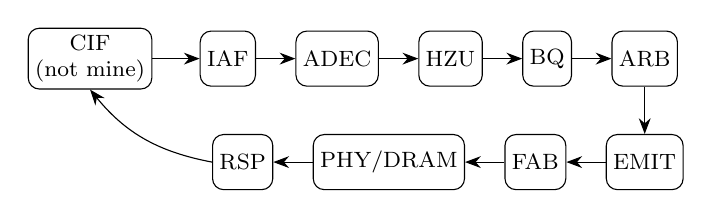
\begin{tikzpicture}[font=\footnotesize,>={Stealth[length=2mm]},
  b/.style={draw,rounded corners,minimum height=7mm,inner sep=2.5pt,align=center}]
  \node[b] (cif) {CIF\\(not mine)};
  \node[b,right=6mm of cif] (iaf) {IAF};
  \node[b,right=5mm of iaf] (adec) {ADEC};
  \node[b,right=5mm of adec] (hzu) {HZU};
  \node[b,right=5mm of hzu] (bq) {BQ};
  \node[b,right=5mm of bq] (arb) {ARB};
  \node[b,below=6mm of arb] (emit) {EMIT};
  \node[b,left=5mm of emit] (fab) {FAB};
  \node[b,left=5mm of fab] (phy) {PHY/DRAM};
  \node[b,left=5mm of phy] (rsp) {RSP};
  \draw[->](cif)--(iaf);\draw[->](iaf)--(adec);\draw[->](adec)--(hzu);
  \draw[->](hzu)--(bq);\draw[->](bq)--(arb);\draw[->](arb)--(emit);
  \draw[->](emit)--(fab);\draw[->](fab)--(phy);
  \draw[->](phy)--(rsp);\draw[->](rsp.west)to[bend left=20](cif.south);
\end{tikzpicture}
\end{center}

\begin{center}\begin{tabular}{@{}llL{6.4cm}@{}}\toprule
Tag & KB name & Role \\ \midrule
IAF & Async REQ FIFO & CIF$\to$core CDC; formed requests in \\
ADEC & AMU (Address Map Unit) & addr $\to$ rank/bg/bank/row/col + align \\
HZU & RAW pause + WR\_TCAM & RAW/WAW/WAR; no-valid-bit gate \\
BQ & Per-Bank In-Flight Queue & 16 FIFOs, head-only, ptr occupancy \\
ARB & Weight Arbiter & FR-FCFS + row-lock + weight + guardrail \\
EMIT & Stage 4 + scoreboard & prove legal, drive CA, advance \sig{next_*} \\
FAB & DFI exchange fabric & pack phases, egress CDC, DFI mux \\
RSP & Async RESP FIFO & tag with \sig{id}, push to CIF \\
ME & Maintenance Engine & peer: refresh/init/zq/rfm/pd/mr (never CAS) \\ \bottomrule
\end{tabular}\end{center}

\textbf{Write path:} IAF $\to$ ADEC $\to$ HZU $\to$ BQ $\to$ ARB $\to$ EMIT $\to$ FAB $\to$
DRAM; ack via RSP. \textbf{Read path:} same to DRAM; data returns FAB.rd $\to$ RSP $\to$
CIF (CIF reorders per \sig{id}, not the core).

%======================================================================
\chapter{MC-Core Architecture (top-level)}

How every block wires together. Two planes: the \textbf{data plane} (solid --- requests to
DRAM, data back) and the \textbf{control/timing plane} (dashed --- scoreboard, maintenance,
gating that decides \emph{when} a command is legal).

\begin{center}
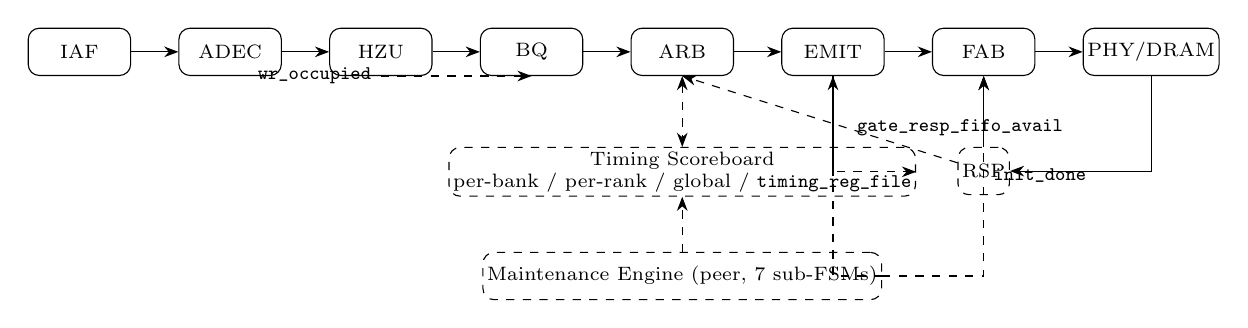
\begin{tikzpicture}[font=\scriptsize,>={Stealth[length=1.8mm]},node distance=6mm,
  d/.style={draw,rounded corners,minimum height=6mm,minimum width=13mm,align=center,inner sep=1.5pt},
  c/.style={draw,dashed,rounded corners,minimum height=6mm,align=center,inner sep=1.5pt}]
  % data plane row
  \node[d](iaf){IAF};
  \node[d,right=of iaf](adec){ADEC};
  \node[d,right=of adec](hzu){HZU};
  \node[d,right=of hzu](bq){BQ};
  \node[d,right=of bq](arb){ARB};
  \node[d,right=of arb](emit){EMIT};
  \node[d,right=of emit](fab){FAB};
  \node[d,right=of fab](phy){PHY/DRAM};
  \draw[->](iaf)--(adec);\draw[->](adec)--(hzu);\draw[->](hzu)--(bq);\draw[->](bq)--(arb);
  \draw[->](arb)--(emit);\draw[->](emit)--(fab);\draw[->](fab)--(phy);
  % control plane row
  \node[c,below=9mm of arb,minimum width=34mm](scb){Timing Scoreboard\\per-bank / per-rank / global / \sig{timing_reg_file}};
  \node[c,below=7mm of scb,minimum width=34mm](me){Maintenance Engine (peer, 7 sub-FSMs)};
  \node[c,below=9mm of fab](rsp){RSP};
  \draw[<->,dashed](arb)--(scb);\draw[->,dashed](emit)|-(scb.east);
  \draw[->,dashed](me)--(scb);\draw[->,dashed](me.east)-|(emit.south);
  \draw[->,dashed](me.east)-|(fab.south) node[pos=0.75,right]{\sig{init_done}};
  \draw[->,dashed](hzu.south)|-(bq.south) node[pos=0.2,left]{\sig{wr_occupied}};
  \draw[->,dashed](rsp)--(arb.south) node[pos=0.4,right]{\sig{gate_resp_fifo_avail}};
  \draw[->](phy.south)|-(rsp.east);\draw[->](rsp.north)--(fab.south);
\end{tikzpicture}
\end{center}

\section{Clock domains}
\begin{center}\begin{tabular}{@{}llL{6.6cm}@{}}\toprule
Domain & Clock & Contains \\ \midrule
CIF & \sig{cif_clk} & AXI slave (not mine) \\
core & \sig{mc_clk} & IAF$\to\ldots\to$EMIT, scoreboard, ME, RSP \\
back-end & \sig{dfi_clk} & FAB, PHY (\sig{dfi_clk}==\sig{mc_clk} baseline $\to$ CDC degenerate) \\ \bottomrule
\end{tabular}\end{center}
Two async-FIFO seams, one real: IAF + RSP are the genuine CDC; the FAB egress CDC collapses
to a register stage at baseline. DRAM \sig{tCK} is hidden PHY-side behind the gear ratio.

\section{Shared-state ownership}
\begin{center}\begin{tabular}{@{}L{5.0cm}L{4.4cm}L{3.4cm}@{}}\toprule
State & Owner (writes) & Readers \\ \midrule
per-bank / global timing tables & EMIT Stage-4 (+ME gates) & ARB, EMIT \\
per-rank FSM table & ME & ARB, EMIT, ME \\
\sig{timing_reg_file} & CSR init + ME MR\_Write & all \\
WR\_TCAM / \sig{wr_occupied} & HZU / watermark mgr & HZU, BQ evict gate \\
per-bank queues & watermark mgr & ARB (head only) \\
bank activity counter & BQ alloc/retire & ME, power-mgmt \\
\sig{gc} & free-running & all \\
\sig{init_done} & ME (one-way latch) & FAB mux \\ \bottomrule
\end{tabular}\end{center}

\section{Config / sizing (validated)}
\sig{N_RD_ENTRIES}=32, \sig{N_WR_ENTRIES}=96 (OW-7 sweep); \sig{bankDepth}=8, \sig{tcam}=32,
in-flight $\le$128 (OQ-20); arbiter control 2/1/0, K=5000, guardrail ON, servo OFF,
\sig{AGE_MAX}=256; \sig{N_RANKS} 1$\to$2 intent; gear 1:1$\ldots$1:4. All pkg values are
\textbf{design intent} --- frozen until RTL-go.

%======================================================================
\chapter{IAF --- Ingress Async Request FIFO}

Upstream boundary. Requests cross the CIF clock into \sig{mc_clk} \textbf{already formed}.
The one real async FIFO (the DFI side is synchronous baseline).

\section{Packet format}
\begin{lstlisting}
req_type 1b            0=RD, 1=WR
axi_id   [AXI_ID_WIDTH] rides through the core, returns with the response
addr     [ADDR_WIDTH]   byte address (ADEC maps it)
size     [BURST_WIDTH]  8/16/32/64/128 B
len      [AWLEN_WIDTH]  burst length (CIF pre-split to BL16 granules)
data     [DATA_WIDTH]   WR only
mask     [STRB_WIDTH]   WR only
\end{lstlisting}
The \sig{axi_id} is the core's only ordering handle --- carried through, handed back so
CIF (not the core) does AXI R/B reordering.

\section{Req vs data split \& CDC}
Descriptor and write payload ride \textbf{parallel async FIFOs} so a stalled data path
never blocks descriptor flow. Credit-based push, KB \S4:
\begin{lstlisting}
CIF write : FIFO_DEPTH credits at init; send when local_credit>0; no comb wr_full
MC read   : rd_valid+rd_data (registered); credit_return -> CIF (1b, MC->CIF sync)
\end{lstlisting}
If \sig{mc_clk}==\sig{cif_clk} the FIFO collapses to a register stage --- kept
parameterized so async is a config change. \sig{FIFO_DEPTH} default 16.

%======================================================================
\chapter{ADEC --- Address Decode / Map Unit (AMU)}

Maps an AXI byte address to \sig{{rank,bg,bank,row,col}} + sub-block offset. Combinational,
setup-time configurable, locked before \sig{init_done}. \textbf{Bank/BG diversity is the
fuel} for datapath-busy; the hash spreads accesses, the extract preserves locality.

\section{Pipeline (2 stages, combinational)}
\begin{lstlisting}
Stage 1  hashed = raw XOR (raw >> xor_shift[field])   if hash_en[field]
Stage 2  field extract from hashed_addr (split fields supported for ch interleave)
\end{lstlisting}

\section{Field assignment (locked, KB \S12)}
\begin{center}\begin{tabular}{@{}lcL{8.2cm}@{}}\toprule
Field & \sig{hash_en} & Rationale \\ \midrule
rank & 1 (MSB) & spread across ranks; rank-switch penalty $\to$ MSB \\
ch & 1 & spread across channels \\
bg & 0 & preserve locality --- row-hit rate critical \\
bank & 0 & preserve locality \\
row & 0 & preserve locality \\
col & 0 & preserve locality; \sig{split_en} for ch interleave \\ \bottomrule
\end{tabular}\end{center}

\section{Sub-block offset + baseline map (32b, 4GB)}
From \sig{size} (8/16/32/64/128 B): \sig{offset[2:0]} + aligned base (mentor's
\sig{Attmem=offset[2:0]} + LSB align). BL16 on the 32b subchannel = 64 B granule.
\begin{lstlisting}
A[31:17]=Row  A[16:14]=BG(3b,8)  A[13:12]=Bank(2b,4)  A[11:2]=Col(10b)  A[1:0]=Offset
Channel = A[7] (128 B interleave baseline)
\end{lstlisting}
\note{\textbf{N\_RANKS 1$\to$2 intent (C1):} rank field non-empty for the 2-rank config
(\sig{RANK_BITS} 0$\to$1); deferred to RTL-go. OQ-19b: ch interleave granularity
(4/8/16 KB) needs the \sig{addrmap} sweep.}

%======================================================================
\chapter{HZU --- Hazard Unit (RAW pause)}

Orders a new request against in-flight same-address accesses before the per-bank queues.
\textbf{RAW is a pause, not a bypass} (mentor).

\section{WR\_TCAM / RAW BCAM --- no valid bit}
Full-address exact match \sig{{bg,bank,row,col}}, \sig{N_WR_ENTRIES}. A match is gated by
\sig{wr_occupied} --- decoded from the write buffer's head/tail pointer range --- so a
retired entry never false-matches:
\begin{lstlisting}
raw_hit_vector[i] = cam_match[i] AND wr_occupied[i]     (no per-entry valid bit)
multi-hit winner  = oldest by program order (seqnum) / argmax(age)
\end{lstlisting}

\section{Cases + the pause}
\begin{center}\begin{tabular}{@{}lllL{4.6cm}@{}}\toprule
New & vs & Hazard & Action \\ \midrule
READ & older WRITE & RAW & pause: \sig{blocked}=1, hold until write drains \\
WRITE & older WRITE & WAW & serialize by \sig{seqnum} \\
WRITE & older READ & WAR & read completes first \\
any & no match & --- & non-hazard $\to$ evict to BQ \\ \bottomrule
\end{tabular}\end{center}
\begin{lstlisting}
On RAW hit: set blocked=1 (READ side) -- do NOT evict.
Hold in the admission station until the blocking write retires; then clear + evict.
Cost: the rare RAW read eats the write's latency serially (no forward, no reorder).
\end{lstlisting}
The pause \textbf{retires} the 2nd hold-forward slot, the Merge Unit, and
\sig{merge_pending}/\sig{wdb_entry_idx}. Only one response source remains (DRAM), so
downstream queues stay CAM-free. \sig{raw_block_en} gates \emph{eviction}, not a bypass mux.
Golden-model proxy \sig{{rank,bank,row}} (conservative); RTL uses full key.

\section{Residency}
WR\_TCAM is a \textbf{short admission station}: search + RAW-compare on admission, then
evict clean entries to the per-bank FIFO. The RD pre-filter TCAM is \textbf{retired}
(v1.9.9) --- candidate set = queue heads.

%======================================================================
\chapter{BQ --- Per-Bank In-Flight Queues}

Holds classified, hazard-cleared requests --- one FIFO per bank, arrival order (natural row
locality). Only the \textbf{head} is active. Occupancy = head/tail pointers, no valid bit.

\section{Entry + rules (KB \S9E)}
\begin{center}\begin{tabular}{@{}llL{7.4cm}@{}}\toprule
Field & W & Meaning \\ \midrule
\sig{rw} & 1 & R/W (unified queue + tag; split is a sweep variant) \\
\sig{seqnum} & SEQ & program order (RAW/retire) \\
\sig{bg,bank} & --- & target (carried for emit) \\
\sig{row,col} & --- & target address \\
\sig{state} & 2 & NEED\_PRE/NEED\_ACT/NEED\_CAS/DONE \\
\sig{blocked} & 1 & RAW-held (set at admission) \\ \bottomrule
\end{tabular}\end{center}
\begin{lstlisting}
depth/bank : 8 (swept) ; total in-flight <= 128 ; tcam=32
head-only  : head asserts ready-bit/class -> can_pre/act/cas[16] to arbiter
             next_cas/pre/act TIMERS are per-bank scoreboard (ch. EMIT), not per-entry
advance    : head self-advances state as ACT/PRE/CAS issue; on CAS done -> pop, next head
occupancy  : head/tail ptr + depth + full = relocated watermark -> admission backpressure
             NO valid bit -- head..tail = occupied by construction
\end{lstlisting}

\section{Sizing (OW-7, deferred to sweep)}
KB says \sig{N_WR}=2--3$\times$\sig{N_RD}; the plan says read=write=64. The datapath floor:
to serve a \textbf{row-miss} read at gap-0, PRE must fire $\approx$ \sig{T_RCD}+\sig{T_RP}
$\approx$ 10 bursts ahead --- so depth $\times$ active banks must hold $\ge$10 bursts of
lookahead. Verdict from a sizing sweep, not a guess. Point so far: \sig{bankDepth}=8,
\sig{tcam}=32, in-flight $\le$128.

%======================================================================
\chapter{ARB --- Weight Arbiter}

Picks the next command from the 16 bank heads (+ maintenance via Stage-0). Model-proven
(33/33).

\section{Weight + guardrail}
\begin{lstlisting}
weight(lane) = K*control[lane] + age[lane] + (lane==ACT ? servo_mod : 0)
  control : CAS>ACT>PRE (fixed; sweep pt 2/1/0)
  age     : +1/waiting cycle, 0 on win  (breaks starvation)
  servo   : DQ-occupancy balance (default OFF)
winner = argmax(weight) over legal candidates
ties -> oldest age -> BG-rotate (bg != last_act_bg : tCCD_S 8 < tCCD_L 12)

GUARDRAIL (dominant): dq_free_in==0 AND ready_cas>=1  =>  CAS wins absolutely
\end{lstlisting}
Sweep design point (OQ-20 DONE): \sig{control}=2/1/0, \sig{K}=5000, guardrail ON, servo
default-OFF, \sig{AGE_MAX}=256. Weights are second-order; guardrail + sizing dominate.

\section{$\ge$2-live-BG invariant}
Same-BG CAS pays \sig{T_CCD_L}(rd, 4-tCK bubble)/\sig{T_CCD_L_WR}(wr, 24-tCK bubble);
diff-BG = \sig{T_CCD_S}=8=gapless. The arbiter \textbf{must} keep $\ge$2 bank-groups with a
ready same-direction CAS and ping-pong between them. The \#1 datapath-busy job.

\section{Per-bank row-lock + adaptive batching}
\begin{lstlisting}
row-lock: acquire on ACT; hold while demand[bank][open_row]>0;
          release on drain OR oldest_miss_age>=AGE_MAX
          two-sided cap: when locked & aged out, can_cas also deasserts so the burst
          finishes, tRTP/tWR clears, and the starved miss's PRE force-breaks in.

batching: run a direction; flip on gateLoss>=BL2 OR stall>=tRAS+tRP.
          R->W ~3 tCK cheap; W->R = tWTR+RL 46-64 tCK -> batch. Steer W->R cross-rank
          (different dies skip tWTR, ~42 vs 64).

NOP priority: 1.opportunity REFsb  2.speculative ACT  3.opposite-batch drain  4.true NOP
\end{lstlisting}

%======================================================================
\chapter{EMIT --- Emit Stage + Timing Scoreboard}

Turns "arbiter wants X" into "X is legal at cycle N." Registered \sig{can_*} flags +
\sig{next_*} deadlines; the emit FSM proves, drives, advances.

\section{Scoreboard --- 3 tables + timing\_reg\_file}
Legal iff \sig{can_x}==1, where \sig{can_x = (gc - next_x)[MSB]==0}, precomputed out of the
pick critical path (no subtractor). Tables: per-bank FSM (\sig{state, row_open, next_cas/
pre/act/ref}), per-rank FSM (\sig{next_act_any/pre_any/cas_any/rd_wr/wr_rd/rfc,
faw_window[4], gate_rfc/zq}), global timing (\sig{next_act_bg/cas_bg/wtr_bg/last_act_bg}
per BG, plus \sig{caFree}/\sig{dqFree}). Params in \sig{timing_reg_file} as \sig{T_*}.

\section{Verified timings (DDR5-4800B)}
\begin{center}\begin{tabular}{@{}lrl@{}}\toprule
Param & tCK & Meaning \\ \midrule
\sig{T_RCD}/\sig{T_RP} & 40/40 & ACT$\to$CAS / PRE$\to$ACT \\
\sig{T_RAS}/\sig{T_RC} & 77/117 & min row-open / ACT$\to$ACT bank \\
\sig{T_RTP}/\sig{T_WR} & 18/72 & RD$\to$PRE / write recovery \\
\sig{T_CCD_S}/\sig{T_CCD_L} & 8/12 & CAS diff-BG / same-BG (read) \\
\sig{T_CCD_L_WR} & 48 & WR$\to$WR same-BG (max(32nCK,20ns)) \\
\sig{T_RRD_S}/\sig{T_RRD_L} & 8/12 & ACT diff-BG / same-BG \\
\sig{T_WTR_S}/\sig{T_WTR_L} & 6/24 & WR$\to$RD diff-BG / same-BG \\
\sig{T_FAW}/\sig{T_PPD} & 32/2 & 4-ACT window / PRE$\to$PRE \\
\sig{RL}/\sig{WL} & 40/38 & read / write latency \\ \bottomrule
\end{tabular}\end{center}

\section{Advance on emit (Stage-4 writeback)}
\begin{lstlisting}
ACT : next_cas=gc+T_RCD; next_pre=gc+T_RAS; next_act=gc+T_RC; act_bg=gc+T_RRD_L;
      act_any=gc+T_RRD_S; faw_window<<gc; last_act_bg=gc; row_open=row
PRE : next_act=gc+T_RP; pre_any=gc+T_PPD; row_open=CLOSED
RD  : next_cas=gc+T_CCD_L; cas_bg=gc+T_CCD_L; cas_any=gc+T_CCD_S; dqFree=gc+RL+BL/2;
      next_pre=gc+T_RTP; rd_wr=gc+RL+BL/2+T_RTW
WR  : next_cas=gc+T_CCD_L_WR; cas_bg=gc+T_CCD_L_WR; wtr_bg=gc+T_WTR_L; dqFree=gc+WL+BL/2;
      next_pre=gc+WL+BL/2+T_WR; wr_rd=gc+WL+BL/2+T_WTR
REF : next_rfc=gc+T_RFC1 (REFab) / next_ref=gc+T_RFCsb (REFsb); assert ca_quiesced
all : caFree += cadence   (2N: +=2, 1N: +=1)
\end{lstlisting}

\section{Slack vector A (windows not points)}
Working backward from DQ slot N: \sig{D_ACT=N-T_RCD}, \sig{D_PRE=N-T_RCD-T_RP}. Window
\sig{[max(D_i-A_i, resource_ready), D_i]}. \sig{A={A_PRE,A_ACT,A_CAS,A_REF}} is CSR-tunable;
smallest \sig{A_i} that keeps the CA lane feasible. Lets the emitter hide prep $\approx$10
bursts ahead. CA lookahead budget: 4 CA slots/burst, 1 = next CAS, 3 free.

%======================================================================
\chapter{FAB --- DFI Exchange Fabric}

Serialize/deserialize (core command/burst $\leftrightarrow$ DFI phases per gear ratio),
cross clocks, and hold the DFI CSRs. Gear ratio 1:1$\ldots$1:4 sets phase count \sig{NPH}=G
and word count \sig{NW}=G.

\section{Register classes}
Five: \textbf{static config} (\sig{cfg_freq_ratio, cfg_2n_mode, cfg_dram_density,
cfg_dq_width, cfg_rank_count, cfg_bl_mode, \ldots}); \textbf{timing} (\sig{t_phy_wrlat,
t_phy_wrdata, t_phy_rdlat, t_rddata_en, \ldots} --- these size the buffers); \textbf{status}
(\sig{sts_init_complete, sts_*_buf_level, sts_*_cdc_full, sts_ca_quiesced});
\textbf{update/handshake} (ctrlupd/phyupd/phymstr/freq-change); \textbf{error}
(\sig{err_dfi_error, err_*_cdc_ovf, err_rddata_timeout, err_ca_parity, err_*_crc}).

\section{Buffers + CDC + DFI mux}
CA out (cmd FIFO $\to$ phase packer: 1-cyc vs 2-cyc, 1N/2N spacing $\to$ cs/cke/odt),
WR out (burst buffer holds across \sig{t_phy_wrlat} + launch aligner + underrun guard),
RD in (outstanding tracker + capture + phase unpacker + return router + timeout). CDC:
gray-ptr async FIFOs (command/wrdata/rddata) + 2-flop handshake syncs; degenerate to
register stages at \sig{mc_clk}==\sig{dfi_clk}.
\begin{lstlisting}
DFI output mux (init_done one-way latch):
  init_done=0 -> Init FSM (in the ME) drives DFI      (boot)
  init_done=1 -> scheduler Stage-4 emit drives DFI    (normal)
  set once at boot DONE, never de-asserted; MRR via Stage-0 bypass (no 3rd mux input)
\end{lstlisting}

\section{Core-side contract}
\sig{caFree}/\sig{ca_credit}, \sig{wr_data_push}/\sig{wr_data_ready},
\sig{rd_return}/\sig{rd_tag}/\sig{rd_return_valid}, \sig{maint_quiesce},
\sig{init_complete}, \sig{error_irq}. \emph{The scheduler schedules commands; the fabric
makes them DFI phases.}

%======================================================================
\chapter{RSP --- Response Route + Egress RESP FIFO}

Takes read data (from FAB) and write acks (from commit), tags with \sig{axi_id}, pushes to
CIF. Thin --- CIF owns AXI R/B ordering.

\section{Packet + sources}
\begin{lstlisting}
resp_type 2b  00=RD_DATA 01=WR_ACK 10=ERR
axi_id  [AXI_ID_WIDTH] ; data [DATA_WIDTH] (RD only) ; status ; last
\end{lstlisting}
Two sources (RD\_DATA from FAB.rd, WR\_ACK from emit), each rate-limited to 1/cycle; a 2:1
arbiter feeds the RESP FIFO. RAW-pause means one data source (DRAM), so the old
Merge/2nd-slot are retired.

\section{Reserved-slot gate (correctness knob)}
\begin{lstlisting}
gate_resp_fifo_avail = (local_credit > reserved_slots)
Every RD reserves a RESP slot at issue; ARB/EMIT must not issue a read unless
gate_resp_fifo_avail==1 -> a landing slot always exists T_PHY_RDLAT later (no overflow,
no read-return deadlock). Reservation clears when data is pushed.
\end{lstlisting}
Credit-based push (MC side), valid-only to CIF (no ready from CIF; MC self-throttles).

%======================================================================
\chapter{ME --- Maintenance Engine (peer)}

Peer to the scheduler, off the packet path. Owns bring-up, refresh, ZQ, RFM, power
management, mode-register traffic, and the DFI mux. \textbf{Never issues a CAS} --- writes
FSM tables + issues its own non-data commands. \sig{init_done} one-way latch.

\section{7 sub-FSMs}
\begin{center}\begin{tabular}{@{}llL{6.4cm}@{}}\toprule
Sub-FSM & Trigger & Issues \\ \midrule
Init & \sig{INIT_KICK} & drives DFI until \sig{init_done} \\
Refresh & credits/\sig{gc} & REF (Stage-0 override) \\
ZQcal & \sig{gc>=next_zqcs} & ZQCAL; \sig{gate_zq} \\
RFM & \sig{raa[b]<=RAAIMT} & RFM \\
PwrMgmt & idle/system & PDE/PDX, SRE/SRX \\
MR\_Poll & \sig{gc>=next_poll_gc} & MRR to MR4 (sideband) \\
MR\_Write & \sig{mr_wr_req} & MRW + verify MRR \\ \bottomrule
\end{tabular}\end{center}

\section{Refresh + MR\_Write}
Refresh: leaky bucket (\sig{ref_credits}+=1/\sig{T_REFI}, $-$=1/REF); \sig{ref_urgent} at
credits$\ge$8. REFab (\sig{gate_rfc}, all banks, \sig{T_RFC1}) / REFsb (one bank,
\sig{T_RFCsb}); target \sig{argmin(bank_act_count)}; opportunity REFsb on NOP. FGR-2x/4x +
MR4 TUF halve \sig{T_REFI}.
MR\_Write (I28): runtime timing changes via shadow$\to$verify-MRR$\to$apply into
\sig{timing_reg_file}; shared MR Read Arbiter (\sig{mrr_requester} tag) with MR\_Poll.
\textbf{Invariant: \sig{timing_reg_file} never out of sync with the DRAM's programmed
latency.}

%======================================================================
\appendix
\chapter{Ideas / Naming / Validation Ledger}

\section{Naming convention}
Params \sig{ALL_CAPS} (\sig{_WIDTH}/\sig{_BITS}/\sig{_DEPTH}, \sig{N_} counts). Deadlines
\sig{next_<event>}; legal flags \sig{can_<event> = (gc-next_x)[MSB]==0}. Scoping \sig{_bg[]}/
\sig{_rank[]}/\sig{_any}. Timing \sig{T_<PARAM>}. Gates \sig{gate_<x>}, \sig{blocked}.
Prefixes \sig{wr_}/\sig{rd_}/\sig{me_cmd_}/\sig{dfi_}/\sig{sched_}/\sig{s0_}. States UPPER.
Commands ACT/CAS\_RD/CAS\_WR/PRE/REFab/REFsb. Progress
NEED\_PRE/NEED\_ACT/NEED\_CAS/DONE. Global cycle \sig{gc}.

\section{Validated design choices (KEEP unless noted)}
\begin{center}\begin{tabular}{@{}L{5.2cm}L{2.4cm}L{5.4cm}@{}}\toprule
Choice & Verdict & Basis \\ \midrule
BL16 only & KEEP & DDR5 native; AXI 64B = 1 BL16 \\
No-valid-bit (ptr occupancy) & KEEP & mentor; swept clean \\
RAW = pause & KEEP & mentor; retires merge/hold-fwd \\
Weight arbiter & KEEP & model: age-led cuts tail \\
Row-hit promotion & KEEP & model: fewer ACTs, holds locality \\
Adaptive batching & KEEP & mentor; partition superseded \\
Registered \sig{can_*} & ADOPT & no subtractor in pick path \\
AMU XOR-hash map & KEEP & bank diversity = fuel \\
Timing wheel & DROP & loses 4--6 pt busy multi-bank \\
RD pre-filter TCAM & DROP & $\to$ queue heads (v1.9.9) \\
Sweep design point & KEEP & OQ-20 (control 2/1/0,K5000,guardrail,AGE\_MAX256,depth8) \\
AXI narrow/excl/QoS & DROP-scope & CIF's job, not the core \\
\sig{N_RANKS} 1$\to$2 & INTENT & cross-rank W$\to$R skips tWTR \\
Read/write depth (OW-7) & \sig{N_RD}=32 \sig{N_WR}=96 & sweep: 3x wins; plan 64/64 worst (busy \& read latency) \\ \bottomrule
\end{tabular}\end{center}

\section{Key harvested ideas}
DQ heartbeat (BL/2=8); $\ge$2-live-BG invariant; R$\to$W/W$\to$R asymmetry; cross-rank
W$\to$R dodges tWTR; 3-free-CA-slots/burst; lookahead depth $\ge$tRCD+tRP ($\approx$10
bursts); slack vector A; backward scheduling; MR\_Write + shared MR Read Arbiter;
valid-credit intra-MC; \sig{gate_resp_fifo_avail} RD-issue gate.

\end{document}
